%% Supplemental Material for:
%% "Flexible neural routing through fluctuation-constrained response geometry"

\documentclass[
  aps,prl,preprint,notitlepage,superscriptaddress,nofootinbib,longbibliography,
  amsmath,amssymb
]{revtex4-2}

\usepackage[utf8]{inputenc}
\usepackage[T1]{fontenc}
\usepackage{graphicx}
\usepackage{booktabs}
\usepackage{bm}
\usepackage{hyperref}
\hypersetup{hidelinks}

\newcommand{\Tr}{\mathrm{Tr}}
\newcommand{\Rey}{\mathrm{Re}}
\newcommand{\Gmax}{G_{\max}^{(2)}}
\newcommand{\Rtask}{\mathcal{R}}
\newcommand{\Cnoise}{\mathcal{C}}
\newcommand{\opnorm}[1]{\left\lVert #1\right\rVert_2}
\newcommand{\frobnorm}[1]{\left\lVert #1\right\rVert_F}

\begin{document}

\begin{center}
{\large\bfseries Supplemental Material\par}
\vspace{0.35em}
{\large\bfseries Flexible neural routing through fluctuation-constrained
response geometry\par}
\vspace{0.8em}
Mingyi Huang$^{1,2}$ and Yuguo Yu$^{1,2}$\par
\vspace{0.35em}
{\small
$^1$Research Institute of Intelligent and Complex Systems, State Key
Laboratory of Medical Neurobiology and MOE Frontiers Center for Brain Science,
and Institute of Science and Technology for Brain-Inspired Intelligence,
Fudan University, Shanghai 200433, China\par
$^2$Shanghai Artificial Intelligence Laboratory, Shanghai 200232, China\par}
\end{center}
\vspace{0.6em}

\begingroup
\small
\sloppy
\tableofcontents
\endgroup

% ============================================================
\section{Definitions and roadmap}
% ============================================================

The Letter follows one hierarchy that should not be conflated.  Flexible
routing is the phenomenon; input--output response geometry is the hidden
computational state; gain supplies controllability on fixed anatomy; and a
stationary fluctuation budget defines a constrained selection problem.  First,
\emph{identifiability}: spontaneous covariance and decay spectra do not fix
response geometry.  Second, \emph{controllability}: diagonal gain can rotate
that geometry; the FlyWire calculation establishes connectome compatibility,
not a measured gain state.  Third, \emph{selection}: the square-zero class
admits an exact finite-budget concentration theorem; a directed mode pair that
is the only nonzero Schur coupling in a stable real-eigenvalue spectrum obeys
an exact onset law, while distributed
Schur coupling has a local quadratic allocation functional.  Fourth,
\emph{orientation}: structured drive predicts a task-to-noise generalized
eigenmode under an explicit cross-term condition; this remains a prospective
biological prediction.  The ALM perturbation analysis tests only
identifiability by asking whether full effective geometry predicts recovery
better than the typical randomly oriented, exact same-spectrum normal control.

The supplement follows this hierarchy.  It gives (i) the gain-gated
construction and full-connectome compatibility test; (ii) the normal
contractive baseline; (iii) exact square-zero stationary cost and propagator
gain; (iv) the fixed-budget selection rule and its onset corollary; (v) the
anisotropic task-to-noise extension; (vi) general-spectrum and higher-order-chain
checks; (vii) the prespecified multi-animal ALM analysis and trained-network
scope checks; and (viii) exact covariance- and spectrum-level ambiguities that
connect the inverse problem to the variational rule.

The main text studies
\begin{equation}
\dot x=Jx+Bu+\xi,\qquad
\langle\xi(t)\xi(t')^\top\rangle=Q\,\delta(t-t'),
\label{eq:s-dynamics}
\end{equation}
with stable generator $J$, stationary covariance
\begin{equation}
J\Sigma+\Sigma J^\top+Q=0,
\label{eq:s-lyapunov}
\end{equation}
background cost
\begin{equation}
\Cnoise_Q(J)=\Tr\Sigma,
\label{eq:s-cost}
\end{equation}
and finite-time response
\begin{equation}
\Rtask_{B,C}(J)=\sup_{t\ge0}\opnorm{Ce^{Jt}B}^2.
\label{eq:s-response}
\end{equation}
The squared worst-case response is
$\Gmax(J)=\sup_t\opnorm{e^{Jt}}^2$.

\subsection{Relation to prior work and precise novelty}

The critical-initialization account of Pachitariu \emph{et al.}\ relates
power-law covariance spectra and near-real DMD modes in spontaneous activity to
critically normalized symmetric random dynamics, then tests memory with fixed
recurrent dynamics and inputs and a trainable readout
~\cite{pachitariu2026critical}.  The present Letter starts from what those
results leave unresolved.  Covariance and DMD eigenvalues constrain variance,
decay and modal rotation, but do not determine a singular input--output map or
how that map changes across states.  Moreover, near-real modes imply low modal
rotation rather than symmetry of the effective operator: the gain-dressed
construction derived below is non-symmetric and non-normal but has an exactly
real spectrum.  We therefore treat critical symmetric dynamics
as a compatible spontaneous scaffold and ask which additional geometry carries
and selects computation.

The ingredients of the Letter connect several established literatures.  Gain
modulation can change selectivity and reorganize activity in a fixed recurrent
network~\cite{zhangabbott2000,stroud2018}; related models use population gating
or low-rank neuromodulation to switch task-relevant representations and
communication routes~\cite{semedo2019,barbosa2023,costacurta2024}.  Hidden
feedforward memory, balanced amplification, and non-normal dynamics already
produce selective transients without near-critical eigenvalues
~\cite{ganguli2008,goldman2009,murphy2009,hennequin2012,hennequin2014,bondanelli2020,christodoulou2022}.
Fixed-eigenspectrum non-normal RNN parameterizations exploit the same freedom to
increase computational expressivity~\cite{kerg2019}.
The trace of a noise-driven stationary covariance is a standard
$\mathcal H_2$-type output-energy measure~\cite{jovanovic2005}, and covariance
spectra have been characterized in random recurrent dynamics
~\cite{hu2022,zavatoneveth2026}.  Recent work has also optimized gain for
stimulus coding under a spiking cost~\cite{pratcarrabin2026}, and
has related representational geometry to task generalization
~\cite{wakhloo2026}.

The Letter does not claim that gain-based routing, hidden feedforward
amplification, $\mathcal H_2$ fluctuation measures, or task/noise whitening are
individually new.  Existing work establishes that directed transient channels
can exist and be controlled.  The present question is how alternative response
geometries are compared once the stable spectrum is fixed and stationary
propagated variance is limited.  The resulting constrained-allocation problem is
\emph{at fixed stable spectrum and under a fixed cap on stationary propagated variance,
which finite-time response geometry is selected?}  The square-zero solution
answers the finite-budget problem exactly within a minimal class; the
single-pair-supported calculation gives an exact onset law within any stable
real-eigenvalue spectrum; and the distributed general-spectrum calculation
derives the local weighted cost geometry.  Structured drive orients the channel
only under the cross-term condition derived below.  The matched gain-state
construction tests controllability, the complete-connectome calculation tests
anatomical compatibility, and ALM perturbations test spectrum insufficiency;
none is an empirical test of budget optimality.  Thus the advance is from a
mechanism that \emph{can} route or amplify to a quantitative price on alternative
response geometries.  Unlike fixed-spectrum RNN parameterizations or
conventional input--output diagnostics, both spectrum and stationary output
energy are constraints rather than performance outcomes.
This also changes the inverse problem: covariance scaling, decay spectra and
nearly real DMD eigenvalues can restrict a class of effective dynamics without
identifying the perturbational singular geometry that determines routing.
Controlled perturbations therefore supply information that spontaneous-only
critical summaries cannot.

The spectral abscissa and numerical abscissa are
\begin{equation}
\alpha(J)=\max_i\Rey\lambda_i(J),\qquad
\omega(J)=\lambda_{\max}\!\left[\frac{J+J^\top}{2}\right].
\end{equation}
Throughout, ``normal'' means $JJ^\top=J^\top J$ for a real operator.
The fixed-budget selection rule concerns
\begin{equation}
J=-aI+K,\qquad a>0,\qquad K^2=0.
\label{eq:s-class}
\end{equation}

% ============================================================
\section{Gain-gated routing with fixed anatomy}
\label{sec:s-gain-routing}
% ============================================================

The biological question in Fig.~1 of the Letter is whether the same anatomical
circuit can change its input--output computation through state-dependent gain
while preserving common spontaneous summaries. A minimal construction answers
this exactly. Let $v$ be one input-population vector and $u_1,u_2$ orthonormal
alternative output-population vectors, with $u_i^\top v=0$.  Thus the two
contexts receive the same input content but assign it to different downstream
readouts. One fixed anatomical matrix contains both output branches,
\begin{equation}
W=(u_1+u_2)v^\top .
\label{eq:s-routing-anatomy}
\end{equation}
Two positive diagonal gain states act on disjoint output populations so that
\begin{align}
K_A=G_AW&=(s_Hu_1+s_Lu_2)v^\top,\\
K_B=G_BW&=(s_Lu_1+s_Hu_2)v^\top,
\label{eq:s-routing-states}
\end{align}
with $s_H>s_L>0$. Both satisfy $K_A^2=K_B^2=0$ and have the same single
nonzero singular value $\sqrt{s_H^2+s_L^2}$. Therefore the generators
$J_A=-aI+K_A$ and $J_B=-aI+K_B$ have identical eigenvalue spectra, identical
stationary covariance eigenspectra under isotropic drive, and identical cost
\begin{equation}
\Tr\Sigma_A=\Tr\Sigma_B
=\frac{N}{2a}+\frac{s_H^2+s_L^2}{4a^3}.
\label{eq:s-routing-cost}
\end{equation}
Their computations differ. At $t=1/a$, the squared transfer through pathway
$i$ in state $\gamma\in\{A,B\}$ is
\begin{equation}
\left|u_i^\top e^{J_\gamma t}v\right|^2
=\left(\frac{s_{i\gamma}}{ae}\right)^2,
\label{eq:s-routing-transfer}
\end{equation}
so exchanging $s_H$ and $s_L$ redirects the same cue toward the alternative
output without changing $W$ or the matched spontaneous spectra. The input
direction remains exactly $v$.  Within the output subspace, the normalized
routed directions are proportional to $s_Hu_1+s_Lu_2$ and
$s_Lu_1+s_Hu_2$; their angle is
\begin{equation}
\theta_{\rm out}=\cos^{-1}\!\left(
\frac{2s_Hs_L}{s_H^2+s_L^2}\right).
\label{eq:s-routing-angle}
\end{equation}

Figure~1 uses $N=40$, $a=1$, $s_H=3$, and $s_L=0.6$. Both states have
$\Tr\Sigma=22.34$ and peak squared gain $1.590$; selected and unselected output
transfer are $1.218$ and $0.0487$, a $25$-fold routing switch, while
$\theta_{\rm out}=67.38^\circ$. The construction
is an exact minimal mechanism, not a claim that cortical context dependence is
limited to square-zero pathways or to gain modulation alone. In a general
recurrent circuit, gain can also move eigenvalues and total variance; matching
those quantities then represents an additional homeostatic constraint rather
than an automatic identity. The exact construction nevertheless makes the key
point: embedded in recurrent anatomy, gain can control the identity of the
amplified population route rather than only its scalar magnitude.

% ============================================================
\section{Connectome-constrained routing on the full FlyWire v783 graph}
\label{sec:s-flywire-routing}
% ============================================================

\subsection{Question, data and scope}

The construction above isolates the mechanism exactly but leaves open whether
route-selective gain can operate when the fixed anatomical substrate is a large,
recurrent biological connectome.  We therefore performed a connectome-constrained
in silico intervention on the full FlyWire materialization-783 release
~\cite{dorkenwald2024} using the v783 connectivity table distributed with the
published whole-brain \emph{Drosophila} model~\cite{shiu2024}.  The published
release contains $139{,}255$ proofread neurons.  Of these, $138{,}639$ occur in
the model connectivity table, which contains $15{,}091{,}983$ directed
neuron-pair edges; the remaining 616 published neurons have no entry in that
table and were appended as zero-edge nodes.  Thus all $139{,}255$ published
neurons and every model edge were retained, without subsetting.

The two sensorimotor routes were taken from the official Shiu et al.
reproduction notebook: (i) 21 right-hemisphere labellar
sugar gustatory receptor neurons to the two bilateral MN9 motor neurons
(feeding), and (ii) 146 published Johnston-organ mechanosensory neurons to the
two DN1/DN2 outputs used for antennal grooming.  Endpoint roots unchanged in
v783 were used directly.  Three roots that changed after v630 were mapped by
stable supervoxel identity in the public Codex label tables:
\begin{itemize}
\item sugar GRN: old root \texttt{720575940620900446}, new root
\texttt{720575940639259967};\\ stable supervoxel \texttt{78818697598428726};
\item MN9: old root \texttt{720575940645521262}, new root
\texttt{720575940618238523};\\ stable supervoxel \texttt{78536329000064308};
\item JON: old root \texttt{720575940626307902}, new root
\texttt{720575940625054647};\\ stable supervoxel \texttt{78536191829712049}.
\end{itemize}
The source repository commit, complete endpoint lists,
mapping table, graph and node-table SHA-256 hashes, and all selected gain-module
IDs are stored in the accompanying machine-readable results.  This is a
connectome-constrained mechanism test, not a reanalysis of measured fly brain
states: the gain fields below are interventions, not observed in vivo gain maps.
The exact inputs can be recreated without redistributing them: the pinned Shiu
repository supplies \nolinkurl{Connectivity_783.parquet}, and the public Codex
v783 \nolinkurl{neurons.csv.gz} supplies the complete ordered set of 139,255
root IDs.  The script
\nolinkurl{validation/prepare_flywire_v783_inputs.py} downloads these files,
verifies their hashes, and generates
\nolinkurl{Completeness_783_all_139255.csv}; immutable URLs, transformations,
and expected SHA-256 values are documented in
\nolinkurl{validation/FLYWIRE_DATA_PROVENANCE.md}.

\subsection{Signed operator and route-defined gain fields}

Let $W_{ij}$ be the signed neurotransmitter-weighted connection count from
presynaptic neuron $j$ to postsynaptic neuron $i$.  To prevent high-outdegree
neurons from setting the global scale, we normalized each nonempty presynaptic
column by its absolute outgoing strength,
\begin{equation}
P_{ij}=\frac{W_{ij}}{\sum_\ell |W_{\ell j}|}.
\label{eq:s-flywire-normalization}
\end{equation}
For each task $t$, unit vectors $b_t$ and $c_t$ mark its published input and
output sets.  Route candidates were selected from unsigned structural
communicability before any signed response was propagated.  With $H=8$ and
$\delta=0.85$, we computed
\begin{align}
f_t&=\sum_{h=1}^{H}\delta^{h-1}|P|^h b_t, &
r_t&=\sum_{h=1}^{H}\delta^{h-1}(|P|^\top)^h c_t,\\
q_t&=\sqrt{f_t\odot r_t}.
\label{eq:s-flywire-corridor}
\end{align}
Inputs and outputs were excluded.  We ranked the remaining neurons by the
route contrast
$d=(q_{\rm feed}-q_{\rm groom})\oslash
(q_{\rm feed}+q_{\rm groom}+\varepsilon\mathbf 1)\odot
\sqrt{q_{\rm feed}+q_{\rm groom}}$, with $\varepsilon=10^{-20}$, and selected
the 256 largest positive scores
for feeding and the 256 largest-magnitude negative scores for grooming as
non-overlapping gain modules.  Thus the
selection used anatomy and published route endpoints, but not the signed task
transfer reported below.

The two states have the same gain histogram: $G_{\rm feed}$ doubles gain only
on the feeding module and $G_{\rm groom}$ doubles gain only on the grooming
module.  The discrete effective propagators are
\begin{equation}
A_s=\beta I+\gamma G_sP,\qquad \beta=0.70,\quad\gamma=0.14.
\label{eq:s-flywire-propagator}
\end{equation}
Because $\|P\|_1\le1$ and $\max_i(G_s)_{ii}=2$, both states obey the same
rigorous stability bound $\|A_s\|_1\le0.98<1$.  This normalization is a
controlled effective-dynamics test, not the nonlinear spiking model of
Ref.~\cite{shiu2024}.

For task $t$ and state $s$, peak route transfer and the two-way routing switch
factor were
\begin{align}
T_{t,s}&=\max_{0\le k\le24}\|C_tA_s^kb_t\|_2^2,\\
S_{\rm route}&=\sqrt{
\frac{T_{\rm feed,feed}}{T_{\rm feed,groom}}
\frac{T_{\rm groom,groom}}{T_{\rm groom,feed}}}.
\label{eq:s-flywire-switch}
\end{align}
Here $C_t$ selects the published output neurons.  We also computed the sparse
spectral radius and the finite-horizon isotropic fluctuation cost
\begin{equation}
C_H(A_s)=\frac{1}{N}\sum_{k=0}^{40}\|A_s^k\|_F^2,
\label{eq:s-flywire-cost}
\end{equation}
using 16 shared Rademacher trace probes, so the two-state difference is estimated
with common random numbers.

The primary null retained the union of the 512 route-corridor neurons and
permuted feeding/grooming labels within joint strata defined by
neurotransmitter sign and separate median splits of log raw out-strength,
normalized in-strength, out-degree, and in-degree.  Separate quantiling avoids
combining quantities on unlike scales; permutation preserves module size, gain
histogram, and the observed label count in every joint covariate stratum while
destroying which corridor receives which state label.  The construction yielded
32 occupied strata, 21 containing both labels; 469 of 512 neurons lay in those
mixed, permutable strata.  The seed ($0$), 999 null permutations and
five acceptance gates were specified in the analysis script: both routes must
prefer their assigned state, $S_{\rm route}$ must exceed the 95th null
percentile with $p\le0.05$, and the two states must differ by less than 2\% in
spectral radius and 5\% in $C_H$.  This gives a minimum attainable corrected
$p$ value of $0.001$.

\begin{figure*}[t]
  \centering
  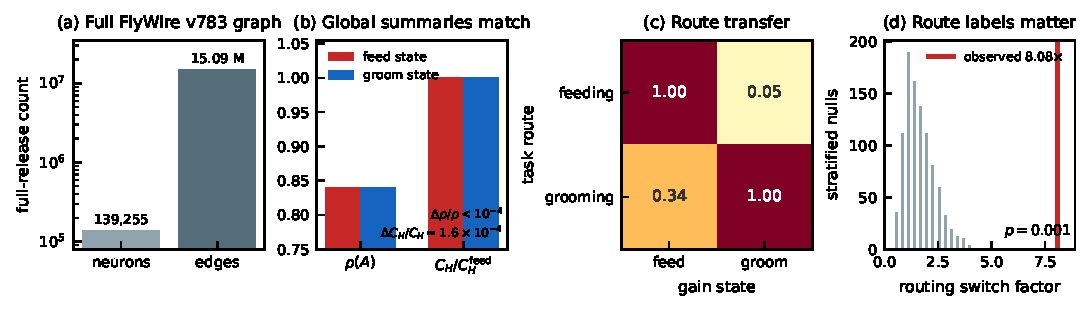
\includegraphics[width=\textwidth]{figures/fig_flywire_gain_routing.pdf}
  \caption{\textbf{Connectome-constrained routing with fixed full-release
  anatomy.} \textbf{(a)} All $139{,}255$ published v783 neurons and all
  $15{,}091{,}983$ directed model edges are retained; 616 neurons absent from
  the connectivity table enter as zero-edge nodes.
  \textbf{(b)} Feeding- and grooming-gain states match in sparse spectral radius
  and finite-horizon fluctuation cost.  \textbf{(c)} Peak task transfer,
  normalized within each route, switches in the predicted direction: feeding
  selectivity is $21.96$ and grooming selectivity is $2.98$.
  \textbf{(d)} Their geometric switch factor is $8.08$, above the
  stratified-null 95th percentile ($3.10$); none of 999 permutations reached or
  exceeded the observed value (corrected one-sided $p=0.001$).  Gain fields are in silico
  interventions; the figure does not establish that flies realize these states
  in vivo.}
  \label{fig:s-flywire-routing}
\end{figure*}

\subsection{Results and sensitivity}

All five acceptance gates passed.  Feeding transfer was $21.96$ times larger
in the feeding state, while grooming transfer was $2.98$ times larger in the
grooming state, giving $S_{\rm route}=8.08$ (Fig.~\ref{fig:s-flywire-routing}).
The stratified-null median and 95th percentile were $1.54$ and $3.10$,
respectively, and none of 999 nulls reached or exceeded the observed value
(corrected one-sided permutation $p=0.001$).  Both sparse spectral-radius
estimates were $0.8400$ at the reported precision; their raw same-solver
relative difference was below $10^{-4}$.  We do not interpret sub-tolerance
digits from the ARPACK calculation (\texttt{tol}$=2\times10^{-4}$): the common
induced-norm bound $\|A_s\|_1\le0.98$ is the rigorous stability guarantee.  The
shared-probe $C_H$ estimates differed by $1.6\times10^{-4}$ in relative terms
($0.016\%$).

We next varied one analysis choice at a time over 13 unique conditions:
gain-module size (128, 256 or 512 neurons), boosted gain (1.5, 2.0 or 2.5),
self-memory $\beta$ (0.60, 0.70 or 0.80), communicability horizon $H$ (4, 8 or
12), damping $\delta$ (0.65, 0.85 or 1.0), and the corridor-ranking rule.  The
two alternative rankings were the raw difference $q_{\rm feed}-q_{\rm groom}$
and $\log[(q_{\rm feed}+\varepsilon)/(q_{\rm groom}+\varepsilon)]$ times the
square root of total corridor strength.  During the gain and $\beta$ sweeps,
$\gamma=(0.98-\beta)/g_{\rm high}$ retained the common induced-norm stability
bound; these are fixed-stability-margin checks rather than unconstrained
parameter sweeps.  Every route-defined switch exceeded its own 95th percentile
from 99 newly generated stratified nulls.  These null ensembles estimate a
robustness threshold rather than define 13 additional inferential endpoints;
the 999-permutation primary test above supplies the reported $p$ value.  Across
the sweep, the switch factor ranged from $3.51$ to $14.98$, and the two-state
finite-horizon-cost difference remained below $0.023\%$.  For the default
ranking, changing the numerical guard from $10^{-12}$ to $10^{-30}$ left both
selected modules unchanged (Fig.~\ref{fig:s-flywire-sensitivity}).

\begin{figure}[t]
  \centering
  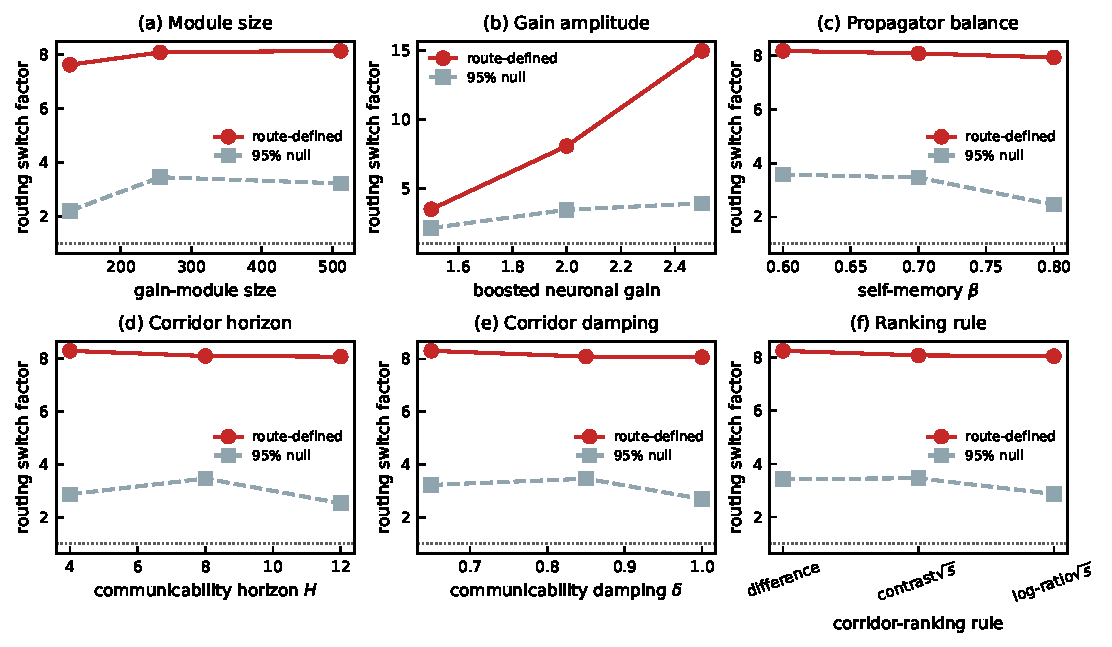
\includegraphics[width=0.98\textwidth]{figures/fig_flywire_gain_routing_sensitivity.pdf}
  \caption{\textbf{Sensitivity of the full-connectome routing test.}
  Route-defined switch factors (red) remain above the 95th percentile of 99
  new stratified nulls per condition (gray) when varying \textbf{(a)} module
  size, \textbf{(b)} gain amplitude, \textbf{(c)} the balance between
  self-memory and propagated input at a common stability bound,
  \textbf{(d)} communicability horizon, \textbf{(e)} communicability damping,
  and \textbf{(f)} corridor-ranking rule.  The central condition is shared
  among panels.}
  \label{fig:s-flywire-sensitivity}
\end{figure}

The result closes a specific gap between the minimal Fig.~1 construction and a
biological wiring diagram: the fixed connectome contains anatomically distinct
sensorimotor corridors that can be selected by equal-size gain fields without a
detectable change in global stability or fluctuation cost.  It does not show
that these gain fields occur naturally, prove that the selected corridor is
optimal among all gain patterns, or validate the fixed-budget theorem in vivo.
A causal test would measure state-dependent gain in the predicted corridor
neurons during feeding versus grooming and ask whether targeted gain
manipulation rotates the perturbational response channel while leaving the
anatomical graph fixed.

% ============================================================
\section{Normal contraction and non-normal onset}
\label{sec:s-normal}
% ============================================================

\subsection{Stable normal operators cannot transiently amplify}

If $J$ is normal, it is unitarily diagonalizable~\cite{trefethen2005},
$J=U\Lambda U^\ast$. Hence
\begin{equation}
\opnorm{e^{Jt}}
=\opnorm{Ue^{\Lambda t}U^\ast}
=\max_i e^{\Rey\lambda_i t}
=e^{\alpha(J)t}.
\end{equation}
For $\alpha(J)<0$, this is at most one for all $t\ge0$, with equality only
at $t=0$. Therefore
\begin{equation}
\Gmax(J)=1.
\end{equation}
For normalized input and readout operators,
\begin{equation}
\opnorm{Ce^{Jt}B}
\le\opnorm{C}\opnorm{e^{Jt}}\opnorm{B}
\le1.
\end{equation}
This establishes the normal bound used in the main text independently of the
stationary-cost budget.

\subsection{What the numerical abscissa does and does not establish}

The Euclidean logarithmic norm satisfies
\begin{equation}
\left.\frac{d}{dt}\right|_{0^+}\opnorm{e^{Jt}}=\omega(J)
\end{equation}
and
\begin{equation}
\opnorm{e^{Jt}}\le e^{\omega(J)t}.
\end{equation}
Thus $\omega(J)\le0$ is sufficient for contraction at every time, while
$\omega(J)>0$ implies initial transient growth. Since
$\alpha(J)\le\omega(J)$, positivity of $\omega-\alpha$ proves that $J$ is
non-normal. The converse is false: a non-normal matrix can have
$\omega=\alpha$. We therefore use the abscissa gap only as a one-sided witness,
not as an equivalence criterion.

% ============================================================
\section{Canonical structure of square-zero coupling}
\label{sec:s-structure}
% ============================================================

\subsection{Orthogonality of input and output subspaces}

For $K^2=0$,
\begin{equation}
\mathrm{range}(K)\subseteq\ker(K).
\end{equation}
The row space of $K$ is $\ker(K)^\perp$. It follows that
\begin{equation}
\mathrm{range}(K)\perp\mathrm{row}(K).
\end{equation}
Let the compact singular-value decomposition be
\begin{equation}
K=USV^\top,\qquad
S=\mathrm{diag}(s_1,\ldots,s_r).
\end{equation}
The columns of $U$ span $\mathrm{range}(K)$ and the columns of $V$ span the
row space, hence
\begin{equation}
U^\top V=0.
\label{eq:s-uvorth}
\end{equation}

\subsection{Orthogonal block form}

Complete the columns of $(U,V)$ to an orthonormal basis. In this basis,
\begin{equation}
K\simeq
\bigoplus_{i=1}^r
\begin{pmatrix}
0&s_i\\
0&0
\end{pmatrix}
\oplus 0_{N-2r}.
\label{eq:s-blockform}
\end{equation}
This is an orthogonal similarity, so it preserves singular values and
Euclidean propagator norms. Since $K$ is nilpotent, all eigenvalues of
$J=-aI+K$ are exactly $-a$, including algebraic multiplicity.

% ============================================================
\section{Exact propagator and stationary covariance}
\label{sec:s-exact}
% ============================================================

\subsection{Matrix exponential}

Because $K^2=0$ and $K$ commutes with $I$,
\begin{equation}
e^{Jt}=e^{-at}e^{Kt}=e^{-at}(I+tK).
\label{eq:s-expm}
\end{equation}
No approximation or truncation error is involved.

\subsection{Isotropic covariance}

For $Q=I$,
\begin{align}
\Sigma
&=\int_0^\infty e^{Jt}e^{J^\top t}\,dt\\
&=\int_0^\infty e^{-2at}
\left[I+t(K+K^\top)+t^2KK^\top\right]dt\\
&=\frac{I}{2a}
+\frac{K+K^\top}{4a^2}
+\frac{KK^\top}{4a^3}.
\label{eq:s-sigma}
\end{align}
The trace of a nilpotent matrix is zero, so
\begin{equation}
\Tr\Sigma
=\frac{N}{2a}+\frac{\Tr(KK^\top)}{4a^3}
=\frac{N}{2a}+\frac{\sum_i s_i^2}{4a^3}.
\label{eq:s-costexact}
\end{equation}
The formula can also be verified by direct substitution into
Eq.~\eqref{eq:s-lyapunov}.

\subsection{Weighted state costs}

A weighted activity cost
\begin{equation}
\Cnoise_{Q,H}(J)=\Tr(H\Sigma H^\top)
\end{equation}
is the squared $\mathcal H_2$ norm from background drive to a weighted output
$y=Hx$~\cite{jovanovic2005}. For the square-zero class,
\begin{align}
\Cnoise_{Q,H}
=\int_0^\infty e^{-2at}
\Tr\!\left[
H(I+tK)Q(I+tK^\top)H^\top
\right]dt .
\end{align}
The isotropic result is recovered with $Q=I$ and $H=I$. Cell-type-specific or
compartment-specific costs therefore change the quadratic metric on $K$ but not
the basic distinction between integrated background cost and finite-time task
response.

% ============================================================
\section{Exact propagator norm}
\label{sec:s-gain}
% ============================================================

For one feedforward block,
\begin{equation}
I+tK_i=
\begin{pmatrix}
1&s_it\\
0&1
\end{pmatrix}.
\end{equation}
The eigenvalues of
$(I+tK_i)^\top(I+tK_i)$ are
\begin{equation}
\lambda_{\pm}
=1+\frac{z^2}{2}\pm\frac{z}{2}\sqrt{z^2+4},
\qquad z=s_it.
\end{equation}
Therefore
\begin{equation}
\opnorm{I+tK_i}^2
=\Phi(s_it),\qquad
\Phi(z)=1+\frac{z^2}{2}
+\frac{z}{2}\sqrt{z^2+4}.
\label{eq:s-phi}
\end{equation}
The derivative
\begin{equation}
\Phi'(z)=z+\frac{z^2+2}{\sqrt{z^2+4}}
\end{equation}
is positive for $z\ge0$. Since the full propagator is a direct sum of these
blocks and scalar decays,
\begin{equation}
\opnorm{e^{Jt}}^2=e^{-2at}\Phi(s_1t),
\end{equation}
where $s_1=\max_i s_i$, and
\begin{equation}
\Gmax=\sup_{t\ge0}e^{-2at}\Phi(s_1t).
\label{eq:s-gainexact}
\end{equation}

% ============================================================
\section{Derivation of the fluctuation-budget selection rule}
\label{sec:s-theorem}
% ============================================================

Fix $a$, $N$, and a stationary-cost cap $C_0\ge N/(2a)$. From
Eq.~\eqref{eq:s-costexact},
\begin{equation}
\sum_i s_i^2\le4a^3\left(C_0-\frac{N}{2a}\right)\equiv S^2.
\label{eq:s-budget}
\end{equation}
For every feasible singular-value vector,
\begin{equation}
s_1\le\left(\sum_i s_i^2\right)^{1/2}\le S,
\end{equation}
with equality throughout exactly when the cap is exhausted and
$s_2=\cdots=s_r=0$. Since
Eq.~\eqref{eq:s-gainexact} is monotonically increasing in $s_1$ at every
$t>0$, its supremum is nondecreasing in $s_1$. Hence a squared-gain maximizer is
\begin{equation}
K_\star=Suv^\top,\qquad \|u\|=\|v\|=1,\qquad u^\top v=0.
\end{equation}
For $S>2a$, every maximizer exhausts the cap and this singular-value allocation
is unique up to zero modes and orthogonal rotations: it yields $\Gmax>1$, and the gain is then
strictly increasing with $s_1$.  For $0<S\le2a$, every feasible allocation is
contractive and ties at $\Gmax=1$ because the supremum occurs at $t=0$; rank
one remains a maximizer but is not selected uniquely.  Orthogonal rotations of
$u$ and $v$ are degenerate under isotropic drive; task and noise statistics
resolve this orientation degeneracy in the anisotropic-drive analysis below.

\subsection{Strict comparison with the normal class}

Every stable normal operator has $\Gmax=1$. The rank-one optimum has
\begin{equation}
\omega(J_\star)=-a+\frac{S}{2}.
\end{equation}
If $S>2a$, then $\omega>0$ and $\Gmax>1$, so no normal operator can solve the
constrained maximization. Using Eq.~\eqref{eq:s-budget},
\begin{equation}
S>2a
\quad\Longleftrightarrow\quad
C_0>\frac{N}{2a}+\frac{1}{a}.
\label{eq:s-threshold}
\end{equation}
If $S\le2a$, then $\omega\le0$ and
$\opnorm{e^{Jt}}\le e^{\omega t}\le1$, so the optimum remains contractive.
Equation~\eqref{eq:s-threshold} is therefore an if-and-only-if threshold within
the square-zero class.  Its relative excess is $2/N$, but its absolute excess is
$1/a$ and does not decrease with network size.  Thus the large-$N$ statement is
subextensive relative to the normal baseline, not a claim that amplification is
absolutely cost-free.

\subsection{Rank-\texorpdfstring{$r$}{r} equal allocation}

If a rank-$r$ allocation exhausts the budget cap, each nonzero singular value is
\begin{equation}
s_r=\frac{S}{\sqrt r}.
\end{equation}
Amplification requires $s_r>2a$, or
\begin{equation}
C_0>\frac{N}{2a}+\frac{r}{a}.
\end{equation}
Thus diffuse coupling requires a proportionally larger excess budget to cross
the same response threshold.

% ============================================================
\section{Anisotropic drive and task--noise alignment}
\label{sec:s-aniso}
% ============================================================

\subsection{Rank-one channel}

Let
\begin{equation}
K=suv^\top,\qquad \|u\|=\|v\|=1,\qquad u^\top v=0.
\end{equation}
For general $Q$,
\begin{align}
\Sigma_Q
={}&\int_0^\infty e^{-2at}
\bigl[Q+st(uv^\top Q+Qvu^\top)\bigr]dt\nonumber\\
&+\int_0^\infty e^{-2at}s^2t^2uv^\top Qvu^\top\,dt .
\end{align}
Taking the trace gives
\begin{equation}
\Cnoise_Q
=\frac{\Tr Q}{2a}
+\frac{s\,u^\top Qv}{2a^2}
+\frac{s^2v^\top Qv}{4a^3}.
\label{eq:s-generalQ}
\end{equation}
The linear cross term shows that, for arbitrary anisotropic $Q$, orientation
selection is not determined by $v^\top Qv$ alone. If $v$ is an eigenvector of
$Q$, $Qv=q_vv$, then
$u^\top Qv=q_vu^\top v=0$, and
\begin{equation}
\Cnoise_Q
=\frac{\Tr Q}{2a}+\frac{s^2q_v}{4a^3}.
\label{eq:s-anisocost}
\end{equation}

The directed transfer is
\begin{equation}
u^\top e^{Jt}v=st\,e^{-at}.
\end{equation}
It peaks at $t_\star=1/a$, yielding
\begin{equation}
\Rtask_{v,u}
=\frac{s^2}{a^2e^2}.
\label{eq:s-transfer}
\end{equation}
Eliminating $s^2$ between Eqs.~\eqref{eq:s-anisocost} and
\eqref{eq:s-transfer},
\begin{equation}
\frac{\Rtask_{v,u}}
{\Cnoise_Q-\Tr Q/(2a)}
=\frac{4a}{e^2q_v}.
\label{eq:s-efficiency}
\end{equation}

\subsection{Multiple orthogonal channels}

Let
\begin{equation}
K=USV^\top
=\sum_i s_i u_iv_i^\top,
\qquad U^\top V=0,
\end{equation}
and assume $Qv_i=q_iv_i$. The excess cost is
\begin{equation}
\Delta\Cnoise
=\sum_i\frac{q_is_i^2}{4a^3}.
\end{equation}
For task weights $r_i\ge0$, define the common-time utility at $t=1/a$,
\begin{equation}
\mathcal U
=\sum_i r_i\left|u_i^\top e^{J/a}v_i\right|^2
=\sum_i\frac{r_is_i^2}{a^2e^2}.
\end{equation}
Writing $z_i=s_i^2$, the allocation problem is linear:
\begin{equation}
\max_{z_i\ge0}\sum_i r_i z_i
\quad\mathrm{s.t.}\quad
\sum_i q_i z_i\le4a^3\Delta C.
\end{equation}
Here and below $Q$ is positive definite on the feasible input subspace, so
$q_i>0$. Without per-channel caps, all budget is allocated to the largest $r_i/q_i$.
With bounds $0\le z_i\le z_i^{\max}$, the solution fills channels in descending
order of $r_i/q_i$. Smooth robustness penalties replace hard filling with a
distributed solution over the same leading ratios.

\subsection{Continuous generalized eigenmodes}

The continuous orientation reduction requires the linear term in
Eq.~\eqref{eq:s-generalQ} to vanish.  This holds automatically for the
eigenvector channels above.  More generally, it holds when the feasible output
subspace contains a unit vector $u$ with $u^\top v=u^\top Qv=0$ (such a choice
exists in an unconstrained space of dimension at least three).  Under this
restriction, assume $Q$ is positive definite on the feasible input subspace.
A unit input direction $v$ then has excess cost
$s^2v^\top Qv/(4a^3)$.  If its task utility is weighted by a positive
semidefinite metric $R$, transfer per excess cost is proportional to
\begin{equation}
\frac{v^\top Rv}{v^\top Qv}.
\end{equation}
Its extrema solve
\begin{equation}
Rv=\lambda Qv.
\end{equation}
The task/noise allocation directions in this reduced quadratic problem are
therefore generalized eigenvectors of the pair $(R,Q)$.  Realizing those directions as
right singular vectors of a dynamical operator remains subject to the
orthogonality and wiring constraints of the feasible set; the statement alone
does not imply global optimality over arbitrary dynamics.  If the cross term
cannot be removed, the full orientation problem must retain its $u$-dependence
and need not reduce to this generalized eigenproblem.

% ============================================================
\section{General-spectrum cost geometry and exact pair onset}
\label{sec:s-general}
% ============================================================

The exact finite-budget selection rule above is restricted to the square-zero
class.  We now separate two statements that generalize from the part that does
not.  First, for any stable spectrum consisting of real eigenvalues, the local
stationary excess cost is a weighted quadratic metric on the Schur
off-diagonal.  Second, a channel supported on any one directed Schur-mode pair
has an exact finite-amplitude cost and onset law.  Distributed coupling is
described only locally by the quadratic metric, whereas the square-zero class
is the minimal locus on which that metric gives the exact finite-budget cost.

\subsection{Reduction to Schur form}
\label{sec:s-schur}

For the real-eigenvalue case used here, write an orthogonal Schur decomposition
\begin{equation}
J=O\,(D+M)\,O^\top,\qquad O^\top O=I,
\label{eq:s-schur}
\end{equation}
with $D=\mathrm{diag}(-a_i)$, $a_i>0$, carrying the fixed stable spectrum and
$M$ strictly upper triangular carrying the Schur off-diagonal. For isotropic
drive $Q=I$ both the stationary cost $\Tr\Sigma$ and the propagator norm
$\opnorm{e^{Jt}}$ are invariant under the orthogonal
conjugation~\eqref{eq:s-schur}, because $O\Sigma O^\top$ solves the transformed
Lyapunov equation and $\opnorm{Oe^{(D+M)t}O^\top}=\opnorm{e^{(D+M)t}}$. Fixing
the real spectrum and maximizing squared gain under a fixed cost cap is therefore equivalent to
fixing $D$ and choosing the strictly upper triangular $M$. A full real Schur form
with complex-conjugate eigenvalue blocks leads to analogous Sylvester equations,
but those blocks are not needed for the analytic extension tested here. No
square-zero assumption is used.

\subsection{Second-order stationary cost for a stable real spectrum}
\label{sec:s-gencost}

Introduce a bookkeeping direction $\widehat M$ through
$J(\varepsilon)=D+\varepsilon\widehat M$ and expand
$\Sigma=\Sigma_0+\varepsilon\Sigma_1+\varepsilon^2\Sigma_2+\cdots$ in the Lyapunov
equation~\eqref{eq:s-lyapunov} with $Q=I$. Matching orders gives
\begin{align}
\Sigma_0&=\mathrm{diag}\!\left(\tfrac{1}{2a_i}\right),
&\Tr\Sigma_0&=\sum_i\frac{1}{2a_i}\equiv C_{\mathrm{normal}},
\label{eq:s-gen0}\\
(\Sigma_1)_{ij}&=\frac{\widehat M_{ij}/2a_j+\widehat M_{ji}/2a_i}{a_i+a_j},
&\Tr\Sigma_1&=0,
\label{eq:s-gen1}
\end{align}
the last equality because $M$ has zero diagonal. The first-order cost of
non-normality vanishes identically: non-normality is a second-order expense. At
second order, the diagonal of $\Sigma_2$ satisfies
$2a_i(\Sigma_2)_{ii}=2(\widehat M\Sigma_1)_{ii}$, and since $\widehat M$ is
strictly upper triangular,
$(\widehat M\Sigma_1)_{ii}=\sum_{k>i}\widehat M_{ik}^2/[2a_k(a_i+a_k)]$.
Writing the actual small Schur off-diagonal as $M=\varepsilon\widehat M$ and
summing gives
\begin{equation}
\Tr\Sigma
=C_{\mathrm{normal}}
+\sum_{i<k} w_{ik}\,M_{ik}^2
+O(\|M\|^3),
\qquad
w_{ik}=\frac{1}{2\,a_i a_k\,(a_i+a_k)}.
\label{eq:s-gencost}
\end{equation}
The stationary cost is a \emph{weighted Frobenius budget} on the Schur
off-diagonal, with a decay-rate kernel $w_{ik}$ that is large for slow
mode pairs and small for fast ones. For a degenerate spectrum $a_i\equiv a$ the
kernel is constant, $w_{ik}=1/4a^3$, so the leading excess cost is the same
Frobenius budget that appears in the square-zero selection rule. The cost formula
of the main text is exact only on the truncation locus discussed below, but its
quadratic part is the degenerate value of this general second-order law.

\subsection{Quadratic general-spectrum allocation functional}
\label{sec:s-genopt}

Near amplification onset, transient growth is equivalent to positivity of the
numerical abscissa $\omega(J)=\lambda_{\max}[\mathrm{Sym}(J)]$.  Write
$S=\mathrm{Sym}(M)=(M+M^\top)/2$, so $S_{ik}=M_{ik}/2$ for $i<k$, and define the
quadratic excess cost
\begin{equation}
\Delta C_2\equiv\sum_{i<k}w_{ik}M_{ik}^2
=4\sum_{i<k}w_{ik}S_{ik}^2.
\label{eq:s-dc2}
\end{equation}
For a fixed unit vector $x$,
\begin{equation}
x^\top(D+S)x=-A(x)+2\sum_{i<k}S_{ik}x_ix_k,
\qquad A(x)=\sum_i a_i x_i^2.
\end{equation}
Weighted Cauchy--Schwarz under Eq.~\eqref{eq:s-dc2} gives
\begin{equation}
2\sum_{i<k}S_{ik}x_ix_k
\le\sqrt{\Delta C_2F(x)},\qquad
F(x)=\sum_{i<k}\frac{x_i^2x_k^2}{w_{ik}},
\label{eq:s-cs}
\end{equation}
with equality for
\begin{equation}
M^\star_{ik}=\frac{\sqrt{\Delta C_2}}{\sqrt{F(x^\star)}}
\frac{x_i^\star x_k^\star}{w_{ik}}.
\label{eq:s-genrankone}
\end{equation}
Maximizing also over $x$ solves the quadratic-cost surrogate exactly,
\begin{align}
\omega_\star^{\rm quad}(\Delta C_2)
&=\max_{\|x\|=1}\left[-A(x)+\sqrt{\Delta C_2F(x)}\right],
\label{eq:s-general-onset}\\
\Delta C_{\rm on}^{\rm quad}
&=\min_{\substack{\|x\|=1\\F(x)>0}}\frac{A(x)^2}{F(x)}.
\label{eq:s-general-threshold}
\end{align}
These equations characterize the local geometry selected by the second-order
Lyapunov metric, not the exact finite-amplitude threshold of the full covariance
problem.  The optimal coupling is generated by one emergent direction
$x^\star$ but can be dense.  Because
$1/w_{ik}=2a_i a_k(a_i+a_k)$, the local cost favors faster mode pairs while
$A(x)$ penalizes their faster intrinsic decay; the outer maximization resolves
this competition.

\subsection{Exact pair-supported onset for an arbitrary stable real-eigenvalue spectrum}
\label{sec:s-pair-exact}

A stronger statement is available when the Schur coupling is supported on one
ordered mode pair.  Restrict the nontrivial block to
\begin{equation}
J_{ik}=\begin{pmatrix}-a_i&m\\0&-a_k\end{pmatrix},
\qquad a_i,a_k>0.
\label{eq:s-pair-generator}
\end{equation}
Solving its Lyapunov equation under isotropic drive gives
\begin{align}
(\Sigma_{ik})_{22}&=\frac{1}{2a_k},\\
(\Sigma_{ik})_{12}&=\frac{m}{2a_k(a_i+a_k)},\\
(\Sigma_{ik})_{11}&=\frac{1}{2a_i}
+\frac{m^2}{2a_i a_k(a_i+a_k)}.
\end{align}
Therefore the stationary excess cost is exactly
\begin{equation}
\Delta C_{ik}=\frac{m^2}{2a_i a_k(a_i+a_k)},
\label{eq:s-pair-exact-cost}
\end{equation}
with no omitted higher-order terms.  The numerical abscissa is the largest
eigenvalue of
$\left(\begin{smallmatrix}-a_i&m/2\\m/2&-a_k\end{smallmatrix}\right)$.
The semigroup is contractive iff this symmetric part is negative semidefinite,
so the onset boundary is
\begin{equation}
m^2=4a_i a_k.
\label{eq:s-pair-onset-m}
\end{equation}
Combining Eqs.~\eqref{eq:s-pair-exact-cost} and
\eqref{eq:s-pair-onset-m} gives the exact law
\begin{equation}
\Delta C_{{\rm on},ik}=\frac{2}{a_i+a_k}.
\label{eq:s-pair-threshold}
\end{equation}
This applies when a single directed pair is the only nonzero Schur coupling,
embedded in any stable spectrum of real eigenvalues, without a small-coupling
approximation.  Onset cost is set by $a_i+a_k$, whereas the required coupling
magnitude is $|m|=2\sqrt{a_i a_k}$; increasing both decay rates lowers the
integrated cost while increasing the required coupling.  For $a_i=a_k=a$,
Eq.~\eqref{eq:s-pair-threshold} gives $1/a$, recovering the square-zero onset.

\subsection{Why the distributed quadratic threshold is not an exact onset law}
\label{sec:s-quad-domain}

For a degenerate spectrum $a_i\equiv a$, the quadratic surrogate has
$A(x)=a$ and $F(x)=2a^3[1-\sum_i x_i^4]$.  Its minimizer is the uniform
direction $|x_i|=N^{-1/2}$, giving
\begin{equation}
\Delta C_{\rm on}^{\rm quad}=\frac{N}{2a(N-1)}
\label{eq:s-degenerate-threshold}
\end{equation}
\emph{for the surrogate}.  It is not the exact finite-amplitude Lyapunov
threshold.  Inserting the uniform optimizer into
Eq.~\eqref{eq:s-genrankone} at this putative onset gives
\begin{equation}
M_{ik}^{\rm quad}=\frac{2a}{N-1}\quad(i<k),\qquad
\frac{\|M^{\rm quad}\|_F}{a}=\sqrt{\frac{2N}{N-1}},
\label{eq:s-quad-norm}
\end{equation}
which is $O(1)$ rather than perturbatively small.  The omitted terms in
Eq.~\eqref{eq:s-gencost} can therefore be comparable to the quadratic term.
The exact Lyapunov calculations in Fig.~\ref{fig:s-general-spectrum}(b,c) show
this upward finite-amplitude departure when $M^2\neq0$.  Thus
Eq.~\eqref{eq:s-degenerate-threshold} diagnoses the distributed direction
preferred by the local metric, not the true finite-amplitude threshold.

\subsection{Square-zero is the cost-truncation locus}
\label{sec:s-truncation}

The exactness of the square-zero result has a structural explanation. For a
degenerate spectrum, $J=-aI+K$ with $K$ nilpotent, the full stationary cost is
\begin{equation}
\Tr\Sigma
=\frac{N}{2a}
+\sum_{\substack{j,l\ge0\\j+l\ge1}}
\frac{(j+l)!}{j!\,l!\,(2a)^{j+l+1}}
\,\Tr\!\big(K^{j}K^{\top l}\big),
\label{eq:s-fullcost}
\end{equation}
obtained by integrating $\frobnorm{e^{Kt}}^2$ term by term. Equivalently, in the
time domain,
\begin{equation}
\frobnorm{e^{Kt}}^2
=N+\|K\|_F^2\,t^2
+t^3 A_3(K)+t^4 A_4(K)+\cdots,
\label{eq:s-integrand}
\end{equation}
where each coefficient beyond the $t^2$ term contains at least one factor
$K^m$ with $m\ge2$; for example $A_4$ contains the positive contribution
$\tfrac14\|K^2\|_F^2$ together with possible mixed terms.  Conversely, if the
nilpotency index is $m+1\ge3$, the highest polynomial term is
$t^{2m}\|K^m\|_F^2/(m!)^2>0$ and cannot cancel. Thus:

\emph{$K^2=0$ is exactly the locus on which the cost functional truncates to the
quadratic budget $\|K\|_F^2/4a^3$.} On that locus the cost-capped problem is
solved in closed form and admits a rank-one maximizer; the singular-value
allocation is selected uniquely once the budget exceeds the amplification
onset. Off that locus
($K^2\neq0$: longer feedforward chains, or dense feedforward graphs), the cost no
longer reduces to a pure Frobenius budget: higher-order polynomial-transient
terms also enter the matched total cost. For the natural higher-order chains
tested in Fig.~2(b) of the Letter and in the numerical implementation section, direct Lyapunov
calculations show that these extra terms do not allow the chains to beat the
square-zero rank-one frontier at matched cost.

The onset comparison makes this concrete. The pure onset ratio $\omega/\|K\|_F$
alone does \emph{not} single out rank one: a fully connected equal-weight feedforward
graph (emergent mode $x^\star$ uniform) attains a slightly larger onset slope.
For example, the $3\times3$ generator $K=\tfrac{1}{\sqrt3}\big(\begin{smallmatrix}
0&1&1\\0&0&1\\0&0&0\end{smallmatrix}\big)$ has $\|K\|_F=1$ and
$\lambda_{\max}(\mathrm{Sym}\,K)=1/\sqrt3\approx0.577>1/2$, exceeding the
rank-one value $1/2$. That generator has $K^2\neq0$, however, so its total
stationary cost is not determined by $\|K\|_F^2$ alone. The optimality of the
rank-one channel above onset is therefore a finite-budget, cost-truncation
property---the regime of Fig.~2 of the Letter---rather than an infinitesimal
onset-slope property.  The two limits do not by themselves identify which
architecture a biological circuit should occupy.  In particular, recurrent
anatomy need not lie near $K^2=0$.  Finite perturbations make a matched-cost
frontier more directly testable than an onset derivative, but this does not
justify imposing the truncation locus.  We therefore use the square-zero solution as
an exact finite-budget benchmark, not as a universal prediction of rank-one
biological connectivity.  The chain and triangle comparisons show that several
natural off-locus motifs remain below that benchmark over the tested cost range,
but they do not solve the generic finite-budget optimization problem.

The weighted second-order cost law~\eqref{eq:s-gencost}, the quadratic
functional~\eqref{eq:s-general-onset}, the exact pair law
~\eqref{eq:s-pair-threshold}, and the finite-amplitude triangle check are tested
against dense Lyapunov solutions in the accompanying verification scripts.

\begin{figure}[!b]
\centering
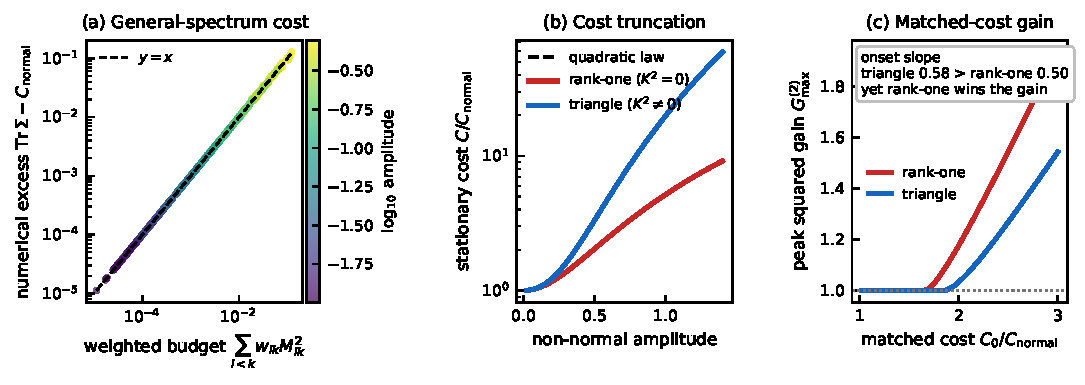
\includegraphics[width=0.95\textwidth]{figures/fig_general_spectrum.pdf}
\caption{\textbf{General-spectrum and off-locus checks.}
(a) For random stable non-degenerate real spectra, the numerical stationary
excess cost $\Tr\Sigma-C_{\rm normal}$ collapses onto the weighted Frobenius
budget of Eq.~\eqref{eq:s-gencost}; color encodes the non-normal amplitude.
(b) The square-zero rank-one channel lies exactly on the quadratic cost law,
whereas a feedforward triangle with $K^2\neq0$ deviates upward at finite
amplitude. (c) Although the triangle has the larger infinitesimal onset slope,
the rank-one square-zero channel dominates the peak squared gain over the
displayed matched-cost range because the triangle pays non-quadratic
polynomial-transient cost.}
\label{fig:s-general-spectrum}
\end{figure}

% ============================================================
\section{Numerical implementation and validation}
\label{sec:s-numerics}
% ============================================================

\subsection{Exact pair-onset checks}

For randomly sampled positive $(a_i,a_k)$, dense Lyapunov solutions reproduce
Eq.~\eqref{eq:s-pair-exact-cost} to numerical precision.  At
$m=2\sqrt{a_i a_k}$, the largest eigenvalue of the symmetric part is zero;
couplings immediately below are contractive and those immediately above have
finite-time squared gain greater than one.  The sampled decay-rate sums and
exact law are stored with the Fig.~2 output.

\subsection{Fixed-budget curves}

The script \texttt{fixed\_budget\_selection.py} evaluates
Eq.~\eqref{eq:s-gainexact} by scalar bounded optimization over time. Parameters
for Fig.~2 of the Letter are
\begin{equation}
N=64,\qquad a=0.2,\qquad
C_{\mathrm{normal}}=\frac{N}{2a}=160.
\end{equation}
For rank $r$ with equal singular values at cost-cap ratio
$\gamma=C_0/C_{\mathrm{normal}}$,
\begin{equation}
s_r=
\sqrt{
\frac{4a^3C_{\mathrm{normal}}(\gamma-1)}{r}
}.
\end{equation}

\begin{table}[t]
\caption{\textbf{Exactly matched non-normal costs under
$C_0/C_{\mathrm{normal}}=1.10$.}
All eigenvalues equal $-0.2$ and all listed costs equal $176$. The normal
reference has cost $160$, is feasible under the same cap, and has squared gain
$\Gmax=1$.}
\label{tab:s-matched}
\begin{ruledtabular}
\begin{tabular}{ccc}
Rank $r$ & largest singular value $s_r$ & squared gain $\Gmax$\\
\midrule
1  & 0.7155 & 2.0392\\
2  & 0.5060 & 1.2222\\
4  & 0.3578 & 1.0000\\
8  & 0.2530 & 1.0000\\
16 & 0.1789 & 1.0000\\
\end{tabular}
\end{ruledtabular}
\end{table}

\subsection{Robustness beyond the minimal response channel}

The main figure also compares the square-zero rank-one frontier with single
higher-order feedforward chains.  For a length-$L$ chain, the nilpotent block
has equal superdiagonal weight $w$ and satisfies $K^L=0$. The stationary cost
is evaluated using the closed form in Eq.~\eqref{eq:s-chaincost}, and the
propagator norm is computed from the exact $L\times L$ block exponential.  The
chains $L=3,4,6$ are then interpolated onto the same
$C_0/C_{\mathrm{normal}}$ grid as the rank-one selection frontier.

Across the displayed range $1\le C_0/C_{\mathrm{normal}}\le1.30$, the maximum
ratio
\begin{equation}
\frac{\Gmax(\mathrm{chain})}{\Gmax(\mathrm{rank\;one})}
\end{equation}
is $1.000$ for $L=3,4,6$, with equality only in the contractive region where
both systems have $\Gmax=1$. Once the rank-one channel crosses the response
threshold, the higher-order chains remain strictly below the frontier.  The
full sweep to $C_0/C_{\mathrm{normal}}=1.6$ is reproduced by
\texttt{higher\_order\_frontier.py} and described again in the
higher-order feedforward-chain extension below.

\subsection{Independent matrix-level check}

For $N=32$, random orthogonal matrices supplied mutually orthogonal $U$ and
$V$, and
\begin{equation}
K=U(sI_r)V^\top.
\end{equation}
We solved Eq.~\eqref{eq:s-lyapunov} with a dense continuous Lyapunov solver and
computed matrix exponentials on a time grid. Results are in
Table~\ref{tab:s-validation}.

\begin{table}[t]
\caption{\textbf{Matrix-level validation at
$C_0/C_{\mathrm{normal}}=1.12$.}
Relative errors compare dense numerical calculations with the closed forms.}
\label{tab:s-validation}
\begin{ruledtabular}
\begin{tabular}{cccc}
Rank & $\frobnorm{K^2}$ & cost relative error & squared-gain relative error\\
\midrule
1 & $1.56\times10^{-17}$ & $4.76\times10^{-16}$ & $1.87\times10^{-6}$\\
3 & $1.99\times10^{-17}$ & $1.59\times10^{-16}$ & $0$\\
8 & $1.89\times10^{-17}$ & $1.59\times10^{-16}$ & $0$\\
\end{tabular}
\end{ruledtabular}
\end{table}

\subsection{Code and reproducibility}

Code, machine-readable outputs, data-provenance records, and instructions for
reproducing all figures and numerical results are archived at
\url{https://github.com/Mia9469/SSNN/tree/prl-routing-submission-v1/Nature_Work/energy_nonnormal}.
Large third-party datasets are not redistributed; the repository provides their
public sources, pinned versions, and integrity checks.

AI-assisted code and manuscript review is disclosed in the Letter.  All
analyses were rerun and checked against the stated derivations and archived
outputs by the authors.

% ============================================================

% ============================================================
\section{Independent multi-animal check: ALM photoinhibition}
\label{sec:s-alm}
% ============================================================

\subsection{Dataset scope and prespecified inclusion rule}

To test the spectrum-insufficiency premise across independent animals, we
analyzed bilateral anterior-lateral motor cortex (ALM) recordings
during unilateral or bilateral photoinhibition~\cite{chen2021modularity,chenli2022dataset}.
The complete Zenodo release is described as 135 sessions from 39 mice.  Its
record page separately exposes 18 session-level
\texttt{data\_structure\_*.mat} files from six mice.  We used all 18 exposed
files and do not treat them as a random or exhaustive sample of the complete
archive.  The file rule, exclusion criteria, windows, latent dimensions and
primary statistic were frozen before the complete 18-file result was inspected
in \texttt{validation/ALM\_ANALYSIS\_PROTOCOL.md}.

Valid trials had a published \texttt{GoodTrials} flag, a finite cue time, no
early lick, one of the two instructed pole locations and photostimulation type
$0$, $1$, $2$ or $3$.  A unit was retained when its manual quality score was
positive and its event-trial coverage spanned the selected task interval.  A
file could be excluded only for prespecified support failures: fewer than 20
such units, fewer than eight non-photostimulation trials for either instructed
location, or fewer than ten variable units after scaling.  Every excluded file
and reason is retained in the machine-readable result rather than selected by
the fitted prediction outcome.

\subsection{Control-only operator and held-condition recovery test}

Spikes were binned at 50 ms and smoothed with a 50-ms Gaussian kernel.  For
each instructed location we subtracted the corresponding control-trial mean
trajectory.  Variable units were standardized from the
control late-delay samples.  The primary basis kept 12 principal components
fit only to those control samples; complete analyses at 8 and 16 dimensions
were prespecified sensitivities.

We fit the one-step latent operator $z_{t+1}=Az_t$ only on
non-photostimulation trials from $-0.85$ to $-0.10$ s relative to the cue,
using ridge regression selected by trial-blocked cross-validation.  The test
set was qualitatively different from the fitting set: unilateral and bilateral
inhibition ended at $-0.90$ s, and the control-trained operator propagated an
early recovery average ($-0.90$ to $-0.75$ s) to a later one
($-0.65$ to $-0.45$ s).  The primary statistic was the Spearman
correlation between predicted and observed log recovery energy after each was
residualized against early log energy.  A stricter sensitivity additionally
removed mean differences among the three photoinhibition types and the two
instructed trial types.

For each fitted $A$, we constructed a real block-normal operator with exactly
the same discrete eigenvalues, including $2\times2$ rotation--dilation blocks
for conjugate pairs.  Random orthogonal conjugations changed its orientation
without changing that spectrum.  Prediction statistics were computed for 200
orientations per session; the surrogate median defined the typical normal
control.  Session statistics were then averaged within each mouse before a
paired one-sided Wilcoxon test; exact sign tests are also reported.  Spectral stability
and transient gain were descriptive and were never used to exclude a file.

Finally, we compared the leading right singular vector of the recovery
propagator with a perturbation-only mode and with a mode generalized by the
control background covariance.  Photoinhibition type does not independently
specify the theorem's task metric or latent drive covariance.  The ALM
alignment and channel-concentration
quantities are therefore exploratory secondary summaries, not tests of the
fixed-budget selection law.

\subsection{Results}

Of the 18 exposed files, 17 passed the prespecified gates and represented all
six mice.  One file was excluded because fewer than 20 stable high-quality
units remained; no file was excluded by stability, gain or prediction.  The
included sessions contained 23--236 variable units and 66--267
photoinhibition trials.  Sixteen of 17 fitted operators had $\rho(A)<1$, and 9
of those 16 showed finite-horizon squared gain above one.  These quantities are
descriptive because the primary comparison does not require or select on a
stable fitted operator.

At the prespecified 12-dimensional resolution, the median across mouse means
was $r_s=0.119$ for full-geometry residual prediction and $0.002$ for the
median same-spectrum normal control, a paired median difference of $0.117$.
The full operator exceeded the surrogate-median control in all six mice (one-sided paired
Wilcoxon $p=0.015625$; exact sign-test $p=0.015625$).  Fourteen of 17 individual
sessions had the same ordering, while only three individual-session statistics
exceeded the 95th percentile of their own 200-control distribution.  The
mouse-level paired result, rather than selectively significant sessions, is the
prespecified inference.  Because six paired mouse values admit only $2^6$
sign patterns, $0.015625$ is the smallest attainable one-sided exact $p$ value
for either primary test.  We therefore treat the paired median difference, the
all-mouse direction, and replication across latent dimensions as the primary
convergence of evidence rather than interpreting the numerical $p$ value as
high-resolution significance.

The stricter condition-adjusted statistic gave median $r_s=0.107$ for full
geometry and $-0.0008$ for controls.  Five of six mouse differences were
positive (Wilcoxon $p=0.03125$; sign-test $p=0.109375$), so this sensitivity is
supportive but weaker than the primary endpoint.  Repeating the complete
primary analysis at 8 and 16 dimensions preserved a positive difference in
all six mice in both cases (full/control medians $0.092/-0.004$ and
$0.123/-0.003$, respectively; Wilcoxon and sign-test $p=0.015625$ for each).

The exploratory orientation test was negative at every resolution: background
weighting improved alignment in $3/6$, $3/6$, and $2/6$ mice at 8, 12, and 16
dimensions, respectively (one-sided Wilcoxon $p=0.281$, $0.656$, and $0.781$).
Leading input-channel concentration was likewise dimension-sensitive.  Its
mouse-median energy fractions versus the isotropic $1/d$ reference were
$0.127/0.125$, $0.096/0.083$, and $0.079/0.0625$ at 8, 12, and 16 dimensions
($p=0.281$, $0.0469$, and $0.015625$).  The latter two nominally positive
comparisons were exploratory, were not prespecified inferential endpoints, and
did not replicate at 8 dimensions; they are reported for completeness rather
than used as evidence for selection.  Neither secondary quantity is used as
ALM evidence for the task/noise allocation law.  The independent positive
conclusion is narrower: a control-trained response geometry predicts recovery
better than typical random normal orientations at the same eigenvalue spectrum.

\begin{table*}[t]
\caption{\textbf{Bilateral-ALM multi-animal scope-check metrics.}
Session values are averaged within mouse before inference.  The primary
endpoint and latent dimensions were fixed before inspection of the complete
18-file result.}
\label{tab:s-alm}
\begin{scriptsize}
\begin{ruledtabular}
\begin{tabular}{lc}
Quantity & Value\\
\midrule
Files exposed / included / excluded & $18/17/1$\\
Included mice / inference unit & $6$ / mouse\\
Stable operators / stable and amplifying & $16/17$ / $9/17$\\
Primary full-geometry residual $r_s$ (mouse median) & $0.119$\\
Primary same-spectrum-normal residual $r_s$ (mouse median) & $0.002$\\
Primary full minus normal / mice positive & $0.117$ / $6/6$\\
Primary one-sided Wilcoxon / exact sign test & $0.015625/0.015625$\\
Strict full / normal residual $r_s$ (mouse medians) & $0.107/-0.0008$\\
Strict mice positive / Wilcoxon / sign test & $5/6$ / $0.03125$ / $0.109375$\\
8-dimensional full / normal; mice positive & $0.092/-0.004$; $6/6$\\
16-dimensional full / normal; mice positive & $0.123/-0.003$; $6/6$\\
Noise weighting, $d=8/12/16$ &
$3/6,3/6,2/6$ mice; $p=0.281/0.656/0.781$\\
Input fraction / $1/d$, $d=8$ & $0.127/0.125$; $p=0.281$\\
Input fraction / $1/d$, $d=12$ & $0.096/0.083$; $p=0.0469$\\
Input fraction / $1/d$, $d=16$ & $0.079/0.0625$; $p=0.015625$\\
\end{tabular}
\end{ruledtabular}
\end{scriptsize}
\end{table*}

\begin{figure*}[t]
  \centering
  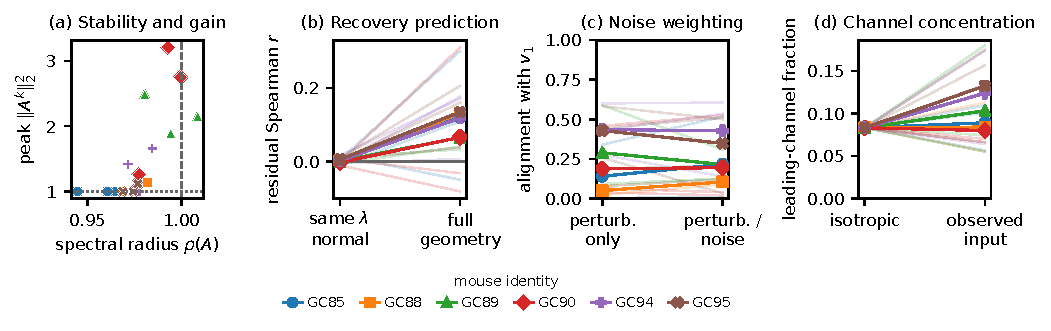
\includegraphics[width=\textwidth]{figures/fig_alm_multisession.pdf}
  \caption{\textbf{Independent bilateral-ALM photoinhibition scope check.}
  Seventeen quality-passing sessions from six mice are shown; one of the 18
  exposed files failed the prespecified unit-support gate.  Colors identify
  mice throughout.  Each faint segment
  represents one included session and each colored segment
  the within-mouse mean.  \textbf{(a)} Fitted control-trial operators are shown
  by spectral radius and peak squared finite-horizon gain; these diagnostics do
  not determine inclusion.  \textbf{(b)} Recovery-energy prediction by the
  full operator is compared with real normal controls having exactly the same
  eigenvalues.  \textbf{(c)} Exploratory alignment of the leading singular
  input with perturbation-only and background-weighted modes.
  \textbf{(d)} Exploratory concentration of early recovery energy in the
  leading input channel relative to the isotropic fraction.}
  \label{fig:s-alm}
\end{figure*}

% ============================================================
\section{Additional empirical scope check: trained recurrent SNNs}
\label{sec:s-empirical}
% ============================================================

\subsection{Purpose and scope}

The trained-network analysis is not used to prove the selection rule.
Its purpose is to test whether the distinctions required by the framework are
material in nonlinear spiking networks:
\begin{enumerate}
\item recurrent connectivity is directed rather than symmetric;
\item bare weights and effective dynamics are different operators;
\item covariance exponents depend on the observed state.
\end{enumerate}
Figure~\ref{fig:s-snn-scope} shows the descriptive empirical anchor across the
two tasks and rate-variance conditions.  The full numerical summary is reported
in Table~\ref{tab:s-snn}.

\subsection{Networks and measurements}

The compiled dataset contains recurrent leaky-integrate-and-fire networks with
$N=512$ trained by surrogate-gradient backpropagation~\cite{neftci2019} on a temporal clusters
task and sequential MNIST. Three random seeds were used for the summary
conditions. Recurrent-weight reciprocity was
\begin{equation}
\eta_W=
\frac{\langle W_{ij}W_{ji}\rangle_{i\ne j}}
{\langle W_{ij}^2\rangle_{i\ne j}}.
\end{equation}
The effective radius was estimated by DMD on realized hidden-state or spike
trajectories. Covariance exponents were fit separately to membrane and
spike-count covariance spectra.

\begin{table*}[t]
\caption{\textbf{Summary of trained SNN measurements.}
Ranges are across three seeds where available. ``Rate-var.'' denotes the
fixed-mean rate-variance condition in the source experiments.}
\label{tab:s-snn}
\begin{ruledtabular}
\begin{tabular}{lcccccc}
Condition
& $\eta_W$
& $\rho(W)$
& $\rho_{\mathrm{eff}}$
& $\nu_{\mathrm{mem}}$
& $\nu_{\mathrm{spike}}$
& seeds\\
\midrule
Clusters baseline
& 0.030--0.031
& 1.59--1.74
& 0.96--0.97
& 0.706--0.823
& 0.340--0.355
& 3\\
Clusters rate-var.
& 0.047--0.052
& 2.01--2.40
& 0.96--0.99
& --- & --- & 3\\
MNIST baseline
& 0.036--0.043
& 3.78--4.51
& 0.96--0.98
& 1.132--1.568
& 0.568--0.735
& 3\\
MNIST rate-var.
& 0.043--0.057
& 3.94--4.54
& 0.97--0.98
& --- & --- & 3\\
\end{tabular}
\end{ruledtabular}
\end{table*}

\begin{figure*}[t]
  \centering
  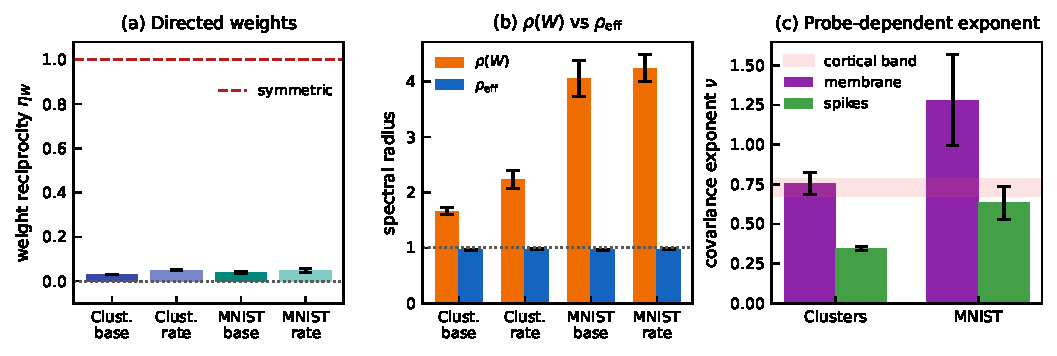
\includegraphics[width=\textwidth]{figures/fig_empirical_anchor.pdf}
  \caption{\textbf{Scope check in trained recurrent spiking networks}
  ($N=512$, three seeds; ``base'' and ``rate-var.'' denote fixed-mean
  rate-variance conditions).  \textbf{(a)} Recurrent weights are strongly
  directed: reciprocity $\eta_W$ stays near zero, far from the symmetric value
  $1$ (dashed).  \textbf{(b)} The bare-weight radius $\rho(W)$ and the
  DMD-fitted effective radius $\rho_{\rm eff}$ are different operators; the
  fitted effective radii remain below unity whereas the bare-weight radii
  exceed unity.  \textbf{(c)} The
  covariance exponent depends on the recorded variable: membrane and spike
  readouts of the same networks give different $\nu$.  This figure anchors
  modeling premises only and does not test non-normal optimality.}
  \label{fig:s-snn-scope}
\end{figure*}

\subsection{Interpretive limits}

Small $\eta_W$ establishes directionality of the recurrent weights, not
non-normal optimality. Likewise, a DMD radius below one establishes stability of
the fitted propagator but does not by itself identify the mechanism that
produces it. The separation between $\rho(W)$ and $\rho_{\mathrm{eff}}$ is
expected because leak, gain, threshold and reset dress the weight matrix.
Moreover, $\rho(W)>1$ is neither a measure of non-normality nor the expansion
parameter in Eq.~\eqref{eq:s-gencost}: it belongs to the bare synaptic matrix,
whereas that perturbative law concerns the Schur off-diagonal of a stable
effective generator.  The trained-network scope check therefore does not place
those networks inside the small-$\|M\|$ regime or test the general-spectrum law
quantitatively.

The membrane/spike difference in $\nu$ demonstrates that a covariance exponent
depends on the observation map. It should therefore be modeled as a statistic
of $(J,Q,C)$ rather than as a structural invariant of $W$.

% ============================================================
\section{Effective dynamics versus synaptic connectivity}
\label{sec:s-effective}
% ============================================================

Linearization of a nonlinear rate network about its operating point gives a
gain-dressed effective generator~\cite{chau2025},
\begin{equation}
J_{\mathrm{eff}}=-I+GW_{\mathrm{syn}}
\quad\text{or}\quad
J_{\mathrm{eff}}=-I+W_{\mathrm{syn}}G,
\qquad G=\mathrm{diag}\,\phi'(x_\star),
\end{equation}
depending on whether the nonlinearity is written before or after recurrent
coupling.  Heterogeneous gain therefore separates effective response geometry
from anatomical reciprocity even in a minimal rate description.

For example, let $W_{\mathrm{syn}}=W_{\mathrm{syn}}^\top$ and $G\succ0$ be
diagonal, and define $S=G^{1/2}W_{\mathrm{syn}}G^{1/2}=S^\top$.  Then
\begin{equation}
GW_{\mathrm{syn}}=G^{1/2}SG^{-1/2},\qquad
W_{\mathrm{syn}}G=G^{-1/2}SG^{1/2}.
\label{eq:s-gain-similarity}
\end{equation}
Both gain-dressed operators have an exactly real spectrum but are generally
non-symmetric and non-normal when $G$ and $W_{\mathrm{syn}}$ do not commute.
Thus near-real fitted modes do not by themselves imply symmetric effective
interactions.  Spiking reset and state-dependent gating add further dressing;
conversely, non-symmetric synaptic connectivity can also yield nearly real
effective modes.

The perturbation susceptibility is similarly dressed:
\begin{equation}
\chi(0)=(-J)^{-1}B.
\end{equation}
Functional covariance, DMD and perturbation response therefore constrain
effective dynamics at a particular operating point. Structural reciprocity
requires connectomics, paired recordings, or an explicit generative model
linking $J$ to $W_{\mathrm{syn}}$.

% ============================================================
\section{From observational ambiguity to variational selection}
\label{sec:s-identifiability}
% ============================================================

The positive selection theory does not require covariance or DMD eigenvalues to
identify a unique generator.  It begins from the opposite premise: observations
define a feasible class of stable effective operators, and response and cost
objectives distinguish members of that class.

The covariance ambiguity is exact even when the drive is known.  For any
$\Sigma\succ0$, $Q\succ0$, and real skew-symmetric $\Omega$, define
\begin{equation}
J_\Omega=\left(-\frac{Q}{2}+\Omega\right)\Sigma^{-1},
\qquad \Omega^\top=-\Omega.
\label{eq:s-covariance-family}
\end{equation}
Every member satisfies
$J_\Omega\Sigma+\Sigma J_\Omega^\top=-Q$ and is Hurwitz because $\Sigma$ is a
positive Lyapunov witness.  Thus even the full stationary covariance, not only
its eigenspectrum, can leave a stable family with different response geometry.
Separately, similar matrices $J_T=TST^{-1}$ have identical eigenvalues but can
have different singular-vector geometry and transient gain when $T$ is
non-orthogonal.  These are complementary ambiguities: covariance and eigenvalue
summaries each leave computational geometry unresolved.

The fixed-budget result does not claim to optimize over either entire
observational equivalence class.  Its claim is conditional and variational:
within an explicitly defined stable fixed-spectrum class, stationary cost and
functional response select structured non-normal effective dynamics.  Nor do
spontaneous functional data by themselves establish non-normal synaptic
connectivity; structural reciprocity remains a separate biological question.

% ============================================================
\section{Falsifiable predictions}
\label{sec:s-predictions}
% ============================================================

The framework makes perturbational predictions that cannot be tested by an
eigenvalue spectrum alone.
\begin{enumerate}
\item \emph{Matched-spectrum response geometry.}  Across behavioral states
with similar DMD eigenvalues and intrinsic timescales, perturbation gain and the
identity of the amplified input should follow the leading singular directions
of the fitted propagator.  States with matched spectra but rotated singular
vectors should route the same perturbation to different population outputs.

\item \emph{Pair-supported onset.}  Approximately pair-supported channels with
real decay rates should obey
$\Delta C_{{\rm on},ik}=2/(a_i+a_k)$ under isotropic fluctuation cost.  Thus
the sum of the decay rates sets the onset cost, whereas their product sets the
required coupling magnitude.  Increasing both rates requires stronger coupling
but lowers integrated excess cost.  This does not assume equal decay rates.

\item \emph{Matched-cost concentration.}  For effective dynamics approaching
the square-zero locus, circuits whose response capacity is concentrated into
fewer directed channels should reach larger finite-time gain than circuits that
distribute the same non-normal strength over many orthogonal modes.  This is a
finite-budget prediction within that regime, not a claimed ordering over all
recurrent architectures.

\item \emph{Task--noise alignment.}  When the anisotropic-cost cross term can be
removed, amplified right singular vectors should
prefer directions with high evoked relevance relative to ongoing variance, not
simply directions of largest task covariance.  Under controlled anisotropic
background drive, Eq.~\eqref{eq:s-efficiency} predicts an inverse relation
between transfer per excess cost and the background variance along the input
direction.

\item \emph{State-dependent reorientation.}  Attention, arousal or
neuromodulation should rotate perturbational singular directions when task/noise
structure changes, even if common spontaneous covariance and eigenvalue
summaries remain approximately matched.  Paired perturbations before and after
the state change provide the direct test.

\item \emph{Fixed-anatomy gain causality.}  Manipulating neuronal gain can
change effective response geometry without changing anatomical reciprocity,
because $J_{\rm eff}=-I+GW_{\rm syn}$.  In the FlyWire example, gain enhancement
of the route-defined feeding module should preferentially increase sugar-GRN to
MN9 transfer, whereas enhancement of the grooming module should preferentially
increase Johnston-organ to DN1/DN2 transfer.  Failure of this crossed
interaction under matched global activity and stability would falsify the
specific connectome-constrained routing mechanism.
\end{enumerate}

These tests require causal perturbations or singular-vector-level analysis.
Changes in eigenvalues alone are neither required by nor sufficient to confirm
the mechanism.

% ============================================================
\section{Extensions and limitations}
\label{sec:s-extensions}
% ============================================================

The exact results occupy distinct domains.  Finite-budget global optimality is
proved only within the equal-decay square-zero class.  The pair-supported onset
law is exact for a single directed Schur-mode pair in a stable real-eigenvalue
spectrum under isotropic trace cost; it is not a global finite-budget optimum
over distributed coupling.  The distributed general-spectrum functional is
quadratic and local, and complex Schur blocks require a separate extension.
Finally, $\Tr\Sigma$ is an operational $\mathcal H_2$ fluctuation cost rather
than a validated metabolic budget, so another cost metric can reorder channels.

\subsection{Higher-order feedforward chains}

If $K^m=0$ for $m>2$,
\begin{equation}
e^{(-aI+K)t}
=e^{-at}\sum_{j=0}^{m-1}\frac{t^jK^j}{j!}.
\end{equation}
A single length-$L$ feedforward chain---an $L$-dimensional Jordan block of $K$
with equal superdiagonal weight $w$---is the natural structured route outside
the square-zero class. It generates transient polynomials of degree $L-1$ but
spreads its Frobenius budget across $L-1$ superdiagonals. Its stationary cost
has the closed form
\begin{equation}
\Tr\Sigma=\frac{N}{2a}
+\sum_{j=1}^{L-1}(L-j)\,\frac{(2j)!}{(j!)^2}\,
\frac{w^{2j}}{(2a)^{2j+1}},
\label{eq:s-chaincost}
\end{equation}
which we verified against the dense Lyapunov solution to a maximum relative
error of $9\times10^{-16}$. The $L=2$ term recovers
$\Tr\Sigma=N/(2a)+w^2/(4a^3)$.

Figure~\ref{fig:s-higherorder} traces the exact cost--squared-gain frontier of these
chains at the same fixed spectrum $\{-a\}$, $N=64$ and $a=0.2$ used in the main
text. Under the isotropic stationary cost, the tested longer chains do not beat the
square-zero rank-one optimum. At a matched budget
$C_0/C_{\mathrm{normal}}=1.10$ the rank-one channel reaches $\Gmax=2.04$,
whereas the $L=3$, $4$ and $6$ chains reach only $1.38$, $1.09$ and $1.00$, a
$32$--$51\%$ deficit; the $L=2$ chain reproduces the rank-one curve to grid
precision. Concentrating the budget on a single superdiagonal therefore
outperforms these tested higher-index alternatives.

This is not a proof of global optimality. The covariance of a general nilpotent
operator contains mixed terms $K^jQ(K^\top)^k$, so a non-isotropic drive or a
weighted output Gramian changes the quadratic metric on $K$ and can reweight the
comparison. The rank-one result should therefore be read as an exact baseline
that is numerically robust to the most natural structured extension, not as a
universal optimum over all directed graphs and cost metrics. The frontier is
reproduced by \texttt{higher\_order\_frontier.py} and
\texttt{higher\_order\_frontier\_results.json}.

\begin{figure}[t]
\centering
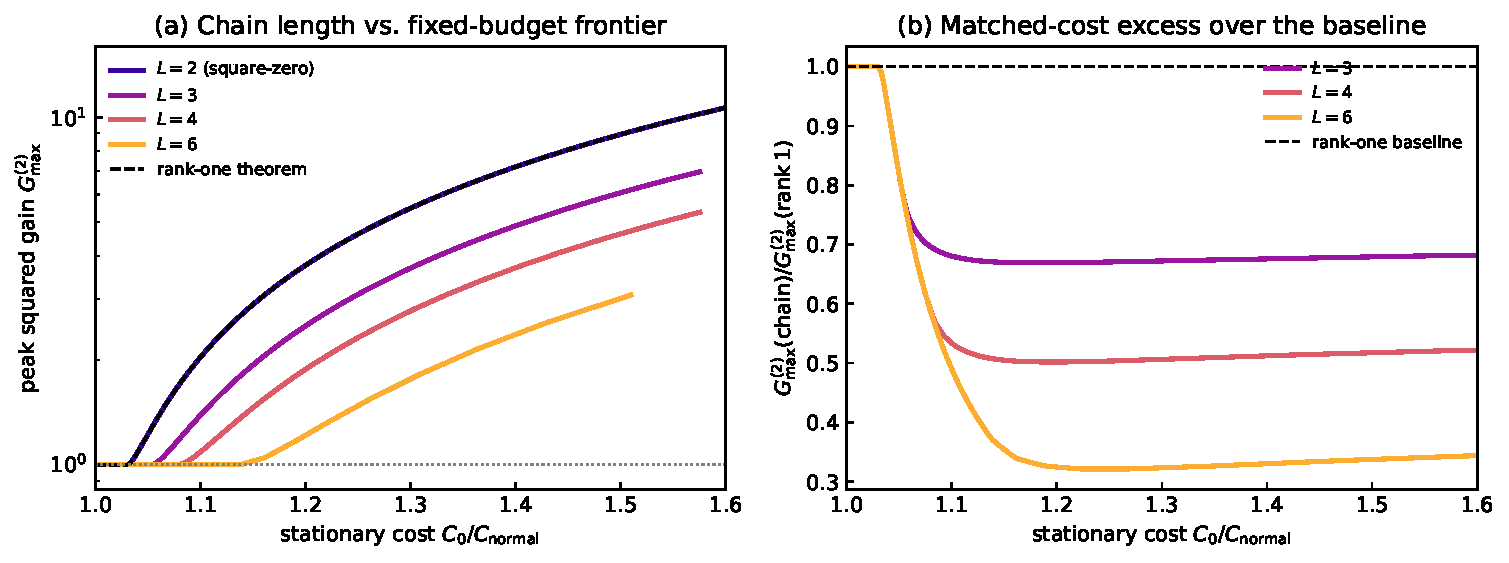
\includegraphics[width=\columnwidth]{figures/fig_higher_order_frontier.pdf}
\caption{\textbf{Tested higher-order feedforward chains do not beat the square-zero
rank-one baseline.} All operators share the spectrum $\{-a\}$ with $N=64$,
$a=0.2$. \textbf{(a)} Exact peak squared gain versus stationary cost for single
feedforward chains of length $L$; $L=2$ is the square-zero rank-one carrier and
coincides with the closed-form selection curve (dashed). \textbf{(b)} Ratio of
chain squared gain to the rank-one optimum at matched cost. Each tested higher-index chain
($L=3,4,6$) lies below unity: spreading response structure across additional
superdiagonals at matched stationary cost reduces peak squared gain.}
\label{fig:s-higherorder}
\end{figure}

\subsection{Dale and sparsity constraints}

Dale's principle constrains columns of $W_{\mathrm{syn}}$, whereas the effective-dynamics rule
is stated for an effective operator. A rank-one effective channel can be
implemented by multi-neuron excitatory/inhibitory motifs even when a literal
rank-one weight matrix violates cell-wise sign constraints. Determining the
minimal Dale-compliant realization is a separate constrained factorization
problem.

\subsection{Nonlinear saturation}

The linear theory predicts onset, early squared gain, and cost around an operating
point. Saturation bounds large responses and can improve robustness, but it also
changes task transfer and stationary activity. A nonlinear extension should
compare its local Jacobian with the analytic frontier while reporting the
finite-amplitude response separately.

\subsection{Alternative cost functions}

Detailed biophysical cost can include firing, synaptic events, membrane
maintenance and cell-type-specific weights. These correspond to different $Q$
and output weighting $H$, or to nonlinear penalties. The task--noise alignment principle
persists whenever background cost is a positive quadratic form in channel
strength and task utility is a different positive quadratic form; the optimal
directions are then generalized eigenmodes of those forms.

\bibliographystyle{apsrev4-2}
\bibliography{references}

\end{document}
